\section{Servizi di un sistema operativo}
I sistemi operativi garantiscono un ambiente in cui eseguire i programmi e fornire servizi, con lo scopo di facilitare l'interazione con i programmatori di applicazioni. Un primo insieme di servizi riguarda funzionalità utili per gli utenti: \begin{itemize}
	\item \textbf{Interfaccia con l'utente}: Meccanismo di interazione fra utente e sistema, si divide in \textbf{interfaccia grafica utente} GUI, \textbf{interfaccia a linea di comando} CLI, e per i dispositivi mobile, \textbf{interfaccia touch-screen}.
	\item \textbf{Esecuzione programmi}: La possibilità di caricare un programma in memoria, eseguirlo e terminarlo.
	\item \textbf{Operazioni I/O}: Il sistema operativo fornisce un’interfaccia uniforme per operazioni di input/output su dispositivi quali dischi, tastiera, schermo e rete.
	\item \textbf{Gestione file system}: Lettura, scrittura e ricerca file, creazione ed eliminazione di directory. Fornisce inoltre i metadati.
	\item \textbf{Comunicazioni}: Scambiare informazioni in uno stesso calcolatore e in diversi elaboratori connessi da una rete.
	\item \textbf{Rilevamento errori}: Rilevazione e segnalazione di errori riguardanti la CPU, dispositivi di memoria, I/O o programmi utente. Gestiti mediante arresto del programma o del sistema, oppure con un codice errore.
\end{itemize}
\noindent Un secondo gruppo invece è atto all'efficienza del sistema: \begin{itemize}
	\item \textbf{Allocazione risorse}: Se più utenti o più processi sono attivi in contemporanea, il sistema operativo provvede alla distribuzione delle risorse necessarie a ciascuno di essi.
	\item \textbf{Accounting}: Mantenere traccia dei programmi usati e quante risorse impiegano.
	\item \textbf{Protezione e sicurezza}: Il sistema operativo evita che i processi interferiscano fra di loro e il sistema stesso e verifica gli utenti tramite richieste di autenticazione.
\end{itemize}
\begin{figure}[h]
	\centering
	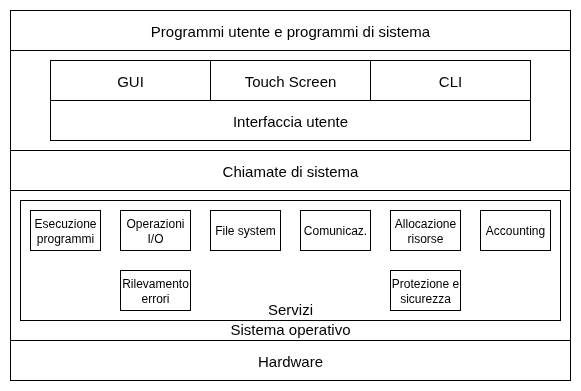
\includegraphics[width=1\linewidth]{Images/OS_services.png}
	\caption{Panoramica dei servizi del sistema operativo}
	\label{fig:OS_services}
\end{figure}

%

\section{Interfaccia utente del sistema operativo}
Ahia le palle

%

\section{Chiamate di sistema}

%

\section{Servizi di sistema}

%

\section{Linker e loader}

%

\section{Struttura del sistema operativo}

%

\section{Generare e avviare un sistema operativo}